\section{System Overview}

The system follows an edge-cloud style architecture with three tiers: the Edge Node, the Central Server, and the Next.js dashboard. The Edge Node performs capture, detection, ROI generation, risk assessment, adaptive encoding, and event buffering. The Central Server ingests streams from multiple cameras, maintains metrics and heatmaps, manages recordings and playback, and serves the dashboard. The dashboard provides live viewing, metric visualization, forensic playback, and privacy controls. This decomposition keeps bandwidth-intensive pixel processing at the edge while centralizing state, storage, and user interaction, consistent with established edge-cloud surveillance designs \cite{Chen2019DIVS,Elgamal2020SIEVE,Nan2023Collaborative}.

[FIGURE PLACEHOLDER --- Figure~5.1: Overall architecture of the proposed adaptive CCTV compression system (deployment view). What to show: Edge Node box (capture, YOLOv8n, ROI, risk, FFmpeg, event buffer) $\rightarrow$ network (UDP/Socket.IO) $\rightarrow$ Central Server box (ingest, metrics, heatmap, recordings, forensic verify) $\rightarrow$ Next.js dashboard box (live, metrics, playback, grid). Purpose: deployment-level visual complement to the pipeline in Figure~4.1. Placement: immediately after this section. Suggested size: 80--90\% of text width. Source: project implementation. Status: NEW FIGURE REQUIRED --- CREATE BEFORE FINAL PRINTING, following the TikZ style of Figure~4.1.]

\section{Edge Node Architecture}

The Edge Node is a Python service built around \texttt{edge-node/capture\_stream.py} with detection abstracted in \texttt{edge-node/detector.py}. Its internal data flow is: camera frame $\rightarrow$ optional CLAHE enhancement $\rightarrow$ YOLOv8n inference (every third frame) $\rightarrow$ ROI merge with 30-frame TTL $\rightarrow$ motion/scene estimation $\rightarrow$ risk scoring (Equation~\ref{eq:risk}) $\rightarrow$ state machine with hysteresis $\rightarrow$ allocation (heuristic path via state-compression table or optimizer path via \texttt{RateAllocator}) $\rightarrow$ FFmpeg encoding with per-state GOP, resolution, and bitrate $\rightarrow$ UDP/Socket.IO transmission plus local event-buffer dumps. Supporting modules include the camera manager, PTZ controller, ReID tracker, audio monitor, and YAMNet classifier, which are present in the repository but outside the evaluated compression path and therefore documented here without evaluation claims.

\section{Risk-State Machine}

\begin{figure}[H]
\centering
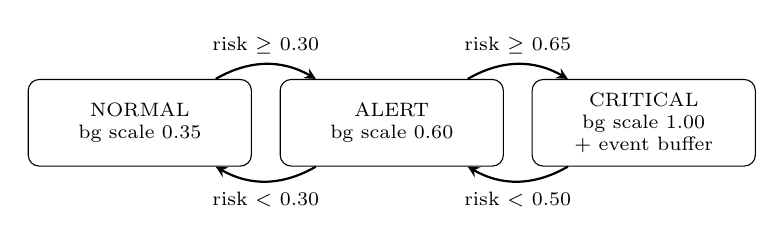
\begin{tikzpicture}[
  node distance=3.2cm, auto,
  state/.style={rectangle, draw, rounded corners, text width=2.6cm, minimum height=1.1cm, align=center, font=\scriptsize},
  arrow/.style={->, >=stealth, thick, font=\scriptsize}
]
\node[state] (n) {NORMAL \\ bg scale 0.35};
\node[state, right of=n] (a) {ALERT \\ bg scale 0.60};
\node[state, right of=a] (c) {CRITICAL \\ bg scale 1.00 + event buffer};
\draw[arrow] (n) to[bend left] node[above] {risk $\geq$ 0.30} (a);
\draw[arrow] (a) to[bend left] node[above] {risk $\geq$ 0.65} (c);
\draw[arrow] (c) to[bend left] node[below] {risk $<$ 0.50} (a);
\draw[arrow] (a) to[bend left] node[below] {risk $<$ 0.30} (n);
\end{tikzpicture}
\caption{Risk-state machine with hysteresis. CRITICAL additionally triggers 15\,s pre-event and 10\,s post-event buffering with forensic manifests.}
\label{fig:state-machine}
\end{figure}

The state machine uses hysteresis (CRITICAL exit at 0.50 versus entry at 0.65) to prevent oscillation at boundaries, with an 8-frame smoothing hysteresis in the live path. State transitions reconfigure GOP length, resolution, compression strength, and frame rate, and CRITICAL additionally opens an event record with server notification.

\section{Central Server Architecture}

The Central Server (\texttt{server/server.js}) is an Express/Socket.IO application accepting per-camera UDP streams. It computes stream metrics every 3000\,ms with automatic bandwidth adaptation (background quality/scale/floor adjusted when measured throughput exceeds twice the 128\,kbps threshold), maintains heatmaps with 300-second decay capped at 10000 points weighted by ROI priority, and exposes REST/Socket endpoints for events, motion, heatmaps, cameras, recordings, playback, reconstruction, and 15-second sample requests with real PSNR/SSIM computation. Recordings are retained on a 7-day hourly rotation. Adaptive streaming rules with exponential moving averaging (factor 0.3), 5-second cooldown, and user-override locking are implemented but disabled by default; this thesis makes no performance claim about them.

\section{Dashboard Architecture}

The dashboard (\texttt{dashboard/src/app}) is a Next.js application with \texttt{live/}, \texttt{metrics/}, \texttt{playback/}, and \texttt{grid/} views plus shared components, configuration, and library layers. It renders live streams, metric time series, heatmap overlays, forensic playback with manifest status, and multi-camera grids, and exposes privacy-mode controls. Screenshots are reserved in Chapter~8.

\section{Configuration Profiles}

Four YAML deployment profiles parameterize the system: \texttt{balanced} (1280$\times$720, 10/20\,fps, hevc\_nvenc p4, 800\,kbps, confidence 0.5), \texttt{high\_quality} (1920$\times$1080, 24/30\,fps, 2000\,kbps, confidence 0.6), \texttt{ultra\_low\_bandwidth} (640$\times$480, 5/10\,fps, 200\,kbps, confidence 0.4), and \texttt{privacy\_mode} (1280$\times$720, 5/15\,fps, 500\,kbps with background blur, face masking, and ethical frame-dropping). Evaluation phases used their own frozen parameters (confidence 0.30, documented per phase) rather than these deployment presets, and the two regimes are not mixed in any reported number.

\begin{table}[H]
\centering
\caption{Deployment configuration profiles (\texttt{configs/*.yaml})}
\label{tab:profiles}
\begin{tabular}{|l|c|c|c|c|}
\hline
\textbf{Profile} & \textbf{Resolution} & \textbf{Bitrate} & \textbf{Conf.} & \textbf{Privacy} \\
\hline
balanced & 1280$\times$720 & 800\,kbps & 0.5 & blur 51 \\
high\_quality & 1920$\times$1080 & 2000\,kbps & 0.6 & off \\
ultra\_low\_bandwidth & 640$\times$480 & 200\,kbps & 0.4 & blur 99 \\
privacy\_mode & 1280$\times$720 & 500\,kbps & 0.5 & blur 99 + mask + ethical drop \\
\hline
\end{tabular}
\end{table}
